\documentclass[conference]{IEEEtran}
% \IEEEoverridecommandlockouts
% The preceding line is only needed to identify funding in the first footnote. If that is unneeded, please comment it out.
\usepackage{cite}
\usepackage{amsmath,amssymb,amsfonts}
\usepackage{algorithmic}
\usepackage{graphicx}
\usepackage{textcomp}
\usepackage{xcolor}
\usepackage{booktabs}
\usepackage{makecell}
\def\BibTeX{{\rm B\kern-.05em{\sc i\kern-.025em b}\kern-.08em
    T\kern-.1667em\lower.7ex\hbox{E}\kern-.125emX}}
\begin{document}

\title{Snek: Development of Deep Q-Learning Agent for Playing the Game of Snake}
\author{\IEEEauthorblockN{1\textsuperscript{st} Guilherme G. Kowalczuk}
\IEEEauthorblockA{\textit{Instituto Tecnológico de Aeronáutica}\\
São José dos Campos, Brazil\\
guilherme.kowalczuk@ga.ita.br}
\and
\IEEEauthorblockN{2\textsuperscript{nd} Jian L. B. Veras}
\IEEEauthorblockA{\textit{Instituto Tecnológico de Aeronáutica}\\
São José dos Campos, Brazil\\
jian.veras@ga.ita.br}
\and
\IEEEauthorblockN{3\textsuperscript{rd} Rina C. Carvalho}
\IEEEauthorblockA{\textit{Instituto Tecnológico de Aeronáutica}\\
São José dos Campos, Brazil\\
rina.carvalho@ga.ita.br}
}

\maketitle


%%%%%%%%%%%%%%%%%%%%%%%%%%%%%%%%%%%%%%%%%%%%%%%%%%%%%%%%%%%%%%%%%%%%%%%%%%%%%%%%
\begin{abstract}

% This electronic document is a ÒliveÓ template. The various components of your paper [title, text, heads, etc.] are already defined on the style sheet, as illustrated by the portions given in this document.

This work presents the implementation of an agent for the game of Snake using Deep Q-Learning. We present the model, state space and reward engineering adopted, as well as the evolution of the agent's performance across training episodes and during evaluation. In this context, the trained agent is consistently capable of scoring at least 10 times per game in 70\% of its games. Lastly, we discuss the results and present conclusions regarding the employed methodology.

\end{abstract}


\section{INTRODUCTION}

First deep learning model to successfully learn control policies from high-dimensional sensory input using Reinforcement Learning (RL) was introduced by DeepMind in 2013. In that paper, they combined classical Deep Learning (DL) algorithms with RL to create a single, general-purpose learning agent that could learn directly from the screen input. The agent was able to learn to play seven Atari 2600 games by only observing the screen pixels and receiving a reward when the game score increased. This study was revolutionary since the agent was able to outperform all previous approaches on six of the games and surpassed a human expert on three of them.

Although Atari was high popular for Millennials and Gen X, the early Gen Z are more familiar with mobile games. One of them is the Snake game, usually played in a Nokia mobile. The game consists of a snake that moves around the screen and increases its score by eating apples and growing in length. The game ends when the snake collides with the borders of the screen or with its own body. The objective of the game is to obtain the highest score possible, which means survive and eat as many apples as possible, without eating its own body. The game of Snake is a good candidate for RL because it is a simple game with a clear reward function and a small state space. Figure \ref{snake-game} shows a illustration of the game.

\begin{figure}[thpb]
   \centering
%    \framebox{\parbox{3in}{We suggest that you use a text box to insert a graphic (which is ideally a 300 dpi TIFF or EPS file, with all fonts embedded) because, in an document, this method is somewhat more stable than directly inserting a picture.
% }}
   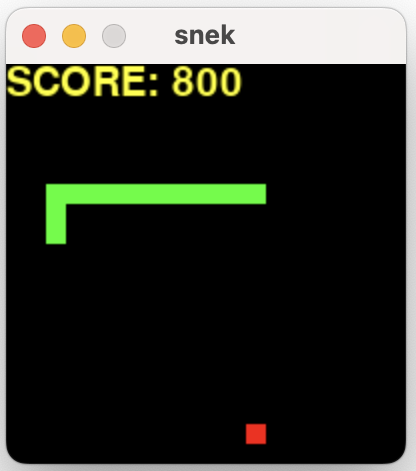
\includegraphics[scale=0.8]{snake-2.png}
   \caption{Snake game from a $20\times20$ grid wall. The main goal for the snake is to eat the apples without eating itself.}
   \label{snake-game}
\end{figure}

In this work, we present the implementation of an agent for the game of Snake using the Deep Q-Learning framework adopted by DeepMind. The main goal is to set up an simulation of the game and train an agent to play it. We present two forms for a state representation and discuss the results obtained by the agent.

\section{DEEP Q-LEARNING}

The Deep Q-Learning algorithm is a combination of Q-Learning and Deep Neural Networks (DNN) that learn complex control policies directly from high-dimensional input. Technically speaking, it consists of a Neural Network model, which can be made of Fully Connected (FC) or Convolutional (Conv) layers, that approximates the action-value function $q(s,a)$. This approximation is necessary because usually the input space-state have a high dimensionality, which makes it impossible to store all the values in a table and apply a Q-Learning algorithm directly.

\subsection{Reinforcement Learning}

A Markov Decision Process is defined as a tuple $(S, A, p, r, \gamma)$. The $S$ is the state-space, which is the set of all possible states. The $A$ stands for the set of possible actions that the agent can execute. $p = p(s'|s, a)$ is the probability that the agent from state $s\in S$ transit to state $s' \in S$ by performing the action $a\in A$. Last but not least, $r = r(s', a, s)$ is the expected reward the agent receives at each step and $\gamma$ is a discount factor.

The RL agent performs a policy $\Pi(a|s)$, which is the probability for an action $a$ taken at each state $s$. For a specific policy $\Pi$, one can define
$$
   v_\Pi(s) = E_\Pi[G_t = R_{t+1} + \gamma R_{t+2} + \cdots | S_t = s],
$$
as the value function, which is the expected cumulative discounted reward by following the policy $\Pi$ from the state $s$. Moreover, one can also define
$$
   q_\Pi(s, a) = E_\Pi[G_t = R_{t+1} + \gamma R_{t+2} + \cdots | S_t = s, A_t = a],
$$
as the action-value function, which is the expected cumulative discounted reward by first taking the action $a$ in the state $S_t = s$, and then following policy $\Pi$ for the next states. The optimal value function $v_*(s)$ and the optimal action-value function $q_*(s, a)$ are defined as the maximum value function and action-value function, respectively, over all possible policies. The optimal policy $\Pi_*$ have the optimal value and action-value function.

\subsection{Q-Learning}

Q-Learning is a off-policy, model-free algorithm which consists on following a policy $\mu$ which is $\epsilon$-greedy, while learning the policy $\Pi$. The $\mu$ policy guarantees that the agent will explore the environment, while the $\Pi$ policy is the one that the agent is learning, which is greedy by construction. The algorithm works by learning the action-value function (represented as $Q(s, a)$, which is different from real $q(s,a)$ function). In each episode, we take the actions $A \sim \mu(a|S)$. In each step from the episode, we take an action and observe the reward $R$ and the next state $S'$. Then, we update the action-value function by
$$
   Q(S, A) \leftarrow Q(S, A) + \alpha \left[ R + \gamma \max_{a'} Q(S', a') - Q(S, A) \right].
$$
In the end of the training, we construct the policy $\Pi$ by taking a greedy policy from learned $Q$. The $\alpha$ is an hyperparameter for the algorithm, and it's actually a smooth factor for the update rule.

\subsection{Q-Learning with Deep Learning}

Usually, many problems have a high-dimensional state space, which makes it impossible to store all the values for $Q$ in a table and apply a Q-Learning algorithm directly. In this case, we can use a Deep Neural Network (DNN) to approximate the action-value function $Q(s, a)$. The DNN is trained by backpropagation and gradient descent. The input of the DNN is the state $s$ and the output is the action-value function $\hat Q(s, a)$. The DNN is trained by minimizing the loss function.

To make the training more stable, we use a technique called Experience Replay. The idea is to store the experiences $(s, a, r, s')$ in a buffer at each step in the episodes, and sample a batch of experiences from it from time to time to train the DNN. This technique is used to break the correlation between the experiences, which makes the training more stable.

Moreover, another technique we use is known as Fixed Q-Targets. The idea is to use a fixed DNN during a mini-batch to estimate the target value $R_{t+1} + \gamma Q(S_t, A_t)$ and ensure the targets don't change during mini-batch. This also makes the training more stable.

\section{METHODOLOGY}

We developed the "Game of Snake" using PyGame, NumPy, Collections in Python. The game architecture is based on three classes: the \texttt{Grid}, which corresponds to the space where the game occurs and also houses the apple (the target for the agent); the \texttt{Agent}, which represents the snake; and the \texttt{Game}, which orchestrates the interactions between the agent and the environment.

There are two game modes: one with closed walls, and the other without. In the first mode, the game-over event happens when the agent touches the borders of the window. However, this event does not occur in the second mode. Another way for the game to end is when the snake's head collides with its body, in both modes. The score increases every time the agent obtains the target (the apple), and a new target is randomly created afterward.

We utilized the Keras framework to implement a deep neural network model designed to evaluate action values. Initially, we employed two distinct models during the training phase: a 2D convolutional neural network (CNN) and a multilayer sequential neural network. However, the sequential model was the first to present convergence. As a result, we decided to proceed with the implementation of the sequential model. The used architecture consists on four dense layers, whose details are presented in Table \ref{tab:NNarchtecture}. The model has mean square error as loss function, and use Adam optimization.

\begin{table}[h]
    \centering
    \label{tab:NNarchtecture}
    \caption{Multilayer sequential neural network architecture}
    \begin{tabular}{cccc} 
        \toprule % Top horizontal line
        Layer & Type & \#Neurons & Activation Function \\
        \midrule % Mid horizontal line
        Input             & -     & \makecell{State vector \\ length (12)} & - \\
        Hidden (1st) & Dense & 128                 & ReLu    \\
        Hidden (2nd) & Dense & 128                 & ReLu    \\
        Hidden (3rd) & Dense & 128                 & ReLu    \\
        Output            & Dense & \makecell{Number of \\actions}   & Linear \\
        \bottomrule % Bottom horizontal line
    \end{tabular}
\end{table}

The agent's state at each instant is represented by a state vector containing 12 boolean variables and serves as the input to the neural network. The first four variables indicate the relative position of the apple to the snake's head (above, below, left, or right). The following four variables describe the presence of an imminent obstacle in relation to the snake's head (above, below, left, or right). Finally, the last four variables specify the snake's current direction (up, down, left, or right). 

Activation functions were chosen in as reported by literature as good choices for the task at hand. The ReLu function is a non-linear function that is easy to compute and has a derivative that is easy to compute. For the output layer, it was chosen the Linear function, instead of Sigmoid function, since the model output has to estimate $Q(S,A)$.


\subsection{Reward Engineering}

In a Deep Q Learning model, the reward mechanism is very important, since it is used to evaluate the agent actions'. Nevertheless, in the case of the snake game, the agent is only rewarded when it catches the apple, so it has no intermediary stimulus to explore the space more efficiently. Then, the reward engineering is required to establish middlemen rewards until the target is attained.

We proposed a reward engineering based on rewarding for catching apple and moving in the direction of the apple, and punishing for dying and getting away from the apple. The values for each recompense is presented in Table \ref{tab:rewards}.

\begin{table}[h]
    \centering
    \label{tab:rewards}
    \caption{Reward engineering schema}
    \begin{tabular}{cc} 
        \toprule % Top horizontal line
        Action & Recompense \\
        \midrule % Mid horizontal line
        Catch apple & +10\\
        Approach the apple & +1 \\
        Move away from the apple & -1 \\
        Die & -100\\
        \bottomrule % Bottom horizontal line
    \end{tabular}
\end{table}

The reward for capturing the apple is significantly lower by a factor of 10 compared to the penalty for encountering the end-state (dying). This design choice aims to promote extended game duration, encouraging the accumulation of at least 10 apples during the agent's gameplay.

The moving direction was set by comparing the distance between snake's head and apple during state transitions. To quantify this distance, the Manhattan distance metric was employed, as the agent's movement is constrained to cardinal directions and does not allow diagonal movement.

Alternative reward metrics, such as session duration and snake length, were taken into consideration. Nonetheless, the rewards presented proved to be effective in achieving convergence during the training process, even with a straightforward model structure.

\section{RESULTS}

We conducted multiple training sessions, with a maximum of 500 sessions each. During these sessions, we tracked the reward history and game score evolution to observe the model's convergence. The first training session took longer to converge as the neural network was being initialized. Subsequent training sets utilized the model file from the previous session, making convergence quicker.

Moreover, all training sessions started with a high epsilon value, following an epsilon scheduling strategy. As a result, each training session began with low reward values that increased gradually over time (faster than the first session).

We executed multiple test sessions to guarantee the model efficiency, since a Deep Q-Learning model has high variance in each execution. For each execution, the epsilon was settled as zero, so the agent could use the greedy policy established with the trained 



\begin{figure}[h]
    \centering
    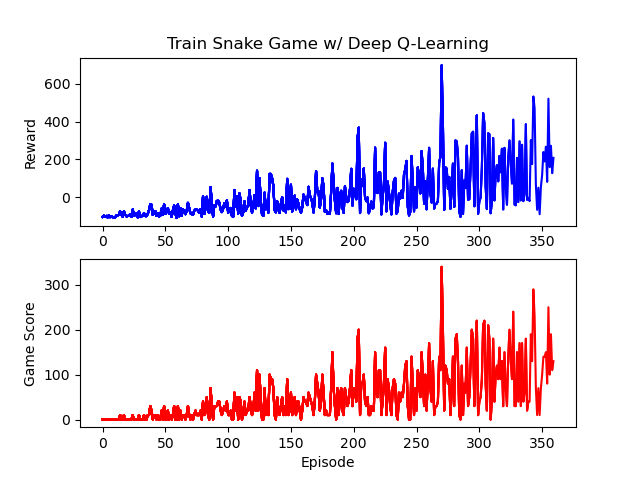
\includegraphics[width=\columnwidth]{dqn_training2.png}
    \caption{Rewards and game scores throughout training.}
    \label{TrainingResults}
\end{figure}

Fig. \ref{TrainingResults} presents an overview of the rewards and game scores through training episodes, in which the agent's performance in the game consistently improves over time, which shows the model is learning an adequate policy for the game. Additionally, Fig. \ref{TestingResults} presents the results for the testing phase, where we can observe the agent has obtained at least 100 points (10 apples) in a game in 25 out of 30 episodes, which is a satisfactory performance. 

\begin{figure}[h]
    \centering
    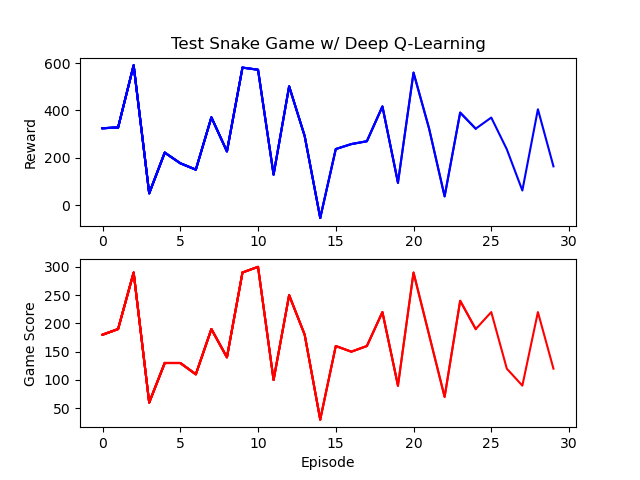
\includegraphics[width=\columnwidth]{dqn_testing.png}
    \caption{Rewards and game scores during evaluation.}
    \label{TestingResults}
\end{figure}




\section{CONCLUSIONS}

In this paper, it was possible to explore Deep Q-Learning algorithm and its application in a real-world problem. The Snake game was perceived as a good candidate for RL because it is a simple game with a clear reward function to test the algorithm. In a first try, the DQL was implemented using a CNN network, which was not able to converge. We suspect that our machines were not powerful enough to train the CNN locally, and it would be necessary to use a high-performance GPU or a paid cloud service to do so. Thus, to overcome this problem, we decided to implement the algorithm using a multilayer sequential neural network and a smaller state space.

Obviously, for such small state space, it would be possible to implement a Q-Learning algorithm directly, without the need of a neural network. However, the main goal of this work was to explore the Deep Q-Learning algorithm, and not to implement a Snake game solver. Indeed, the sequential model was able to converge and learn how to play the snake game after a couple iterations in a reward engineering process. So, we can conclude that the Deep Q-Learning algorithm is a good choice for this kind of problem, and can be used to teach a snake how to eat apples.

\begin{thebibliography}{99}
   \bibitem{DeepMind} Mnih V. \textit{et al.}, "Playing Atari with Deep Reinforcement Learning," in \textit{arXiv:1312.5602 [cs.LG]}, 2013.

   \bibitem{Sebastianelli} A. Sebastianelli, M. Tipaldi, S. L. Ullo and L. Glielmo, "A Deep Q-Learning based approach applied to the Snake game," 2021 29th Mediterranean Conference on Control and Automation (MED), PUGLIA, Italy, 2021.

\end{thebibliography}

\end{document}